\documentclass{beamer}
\usepackage{listings}\usepackage[utf8]{inputenc}
\usepackage[T1]{fontenc}
\usepackage[french]{babel}
\usepackage{listings}
\usepackage{lmodern}
\usepackage{amsmath}
\usepackage{amssymb}
\usepackage{algorithm}
\usepackage{algpseudocode}
\usepackage{array}
\usepackage{pgf,tikz} 
\usepackage{graphicx}
\usepackage{subfig}
\usepackage{media9}
\usetikzlibrary{arrows}


\usetheme{Warsaw}
\title[]{Réseaux de neurones récurrents et LSTM}
\author[Projet long LSTM]{{\footnotesize Maxime Amossé, Vincent Auriau, Laurent Beaughon, Marc Bélicard, Yaqine Héchaïchi, Julien Hemery, Hugo Hervieux, Sylvain Pascou, \newline Thaïs Rahoul, Pierre Vigier \newline encadrés par Arpad Rimmel et Joanna Tomasik}}
\institute{
\includegraphics[scale=0.3]{images/centralesupelec.jpeg}}
\date{7 juin 2017}

\expandafter\def\expandafter\insertshorttitle\expandafter{%
  \insertshorttitle\hfill%
  \insertframenumber\,/\,\inserttotalframenumber}
  
\AtBeginSection[]{
  \begin{frame}
  \vfill
  \centering
  \begin{beamercolorbox}[sep=8pt,center,shadow=true,rounded=true]{title}
    \usebeamerfont{title}\insertsectionhead\par%
  \end{beamercolorbox}
  \vfill
  \end{frame}
}

\AtBeginSubsection[]{
  \begin{frame}
  \vfill
  \centering
    \usebeamerfont{title}\insertsubsectionhead\par%
  \vfill
  \end{frame}
}

\begin{document}

\begin{frame}
\titlepage
\end{frame}

\begin{frame}
Séparation
\end{frame}

\section{Génération de séquences avec des LSTM}

\begin{frame}{Principe}

\end{frame}

\begin{frame}{Exemple : génération de texte}

\end{frame}

\section{Génération de musique}

\begin{frame}{Trois approches différentes}

\end{frame}

\subsection{Génération de spectres audio}

\begin{frame}{Principe}


\end{frame}

\begin{frame}{Résultats}

\end{frame}

\subsection{Génération de midi}

\begin{frame}{Format}
\begin{tiny}
\begin{center}
\begin{tabular}{|c|c|c|c|c|c|c|c|c|c|c|c|c|}
\hline
 & \multicolumn{12}{c|}{\textbf{Hauteurs}} \\
\hline
\textbf{Octave Number} & C & C\# & D & D\# & E & F & F\# & G & G\# & A & A\# & B  \\
\hline
0 & 0 & 1 & 2 & 3 & 4 & 5 & 6 & 7 & 8 & 9 & 10 & 11  \\
\hline
1 & 12 & 13 & 14 & 15 & 16 & 17 & 18 & 19 & 20 & 21 & 22 & 23  \\
\hline
2 & 24 & 25 & 26 & 27 & 28 & 29 & 30 & 31 & 32 & 33 & 34 & 35  \\
\hline
3 & 36 & 37 & 38 & 39 & 40 & 41 & 42 & 43 & 44 & 45 & 46 & 47  \\
\hline
4 & 48 & 49 & 50 & 51 & 52 & 53 & 54 & 55 & 56 & 57 & 58 & 59  \\
\hline
5 & 60 & 61 & 62 & 63 & 64 & 65 & 66 & 67 & 68 & 69 & 70 & 71  \\
\hline
6 & 72 & 73 & 74 & 75 & 76 & 77 & 78 & 79 & 80 & 81 & 82 & 83  \\
\hline
7 & 84 & 85 & 86 & 87 & 88 & 89 & 90 & 91 & 92 & 93 & 94 & 95  \\
\hline
8 & 96 & 97 & 98 & 99 & 100 & 101 & 102 & 103 & 104 & 105 & 106 & 107  \\
\hline
9 & 108 & 109 & 110 & 111 & 112 & 113 & 114 & 115 & 116 & 117 & 118 & 119  \\
\hline
10 & 120 & 121 & 122 & 123 & 124 & 125 & 126 & 127 &   &   &   & \\
\hline
\end{tabular}
\end{center}
\end{tiny}
Commandes :
\begin{itemize}
\item $note\_on \ note \ velocity \ time$
\item $note\_off \ note \ velocity \ time$
\end{itemize}
\end{frame}

\begin{frame}{Principe}
\begin{figure}[!tbp]
  \centering
  \subfloat[Jig]{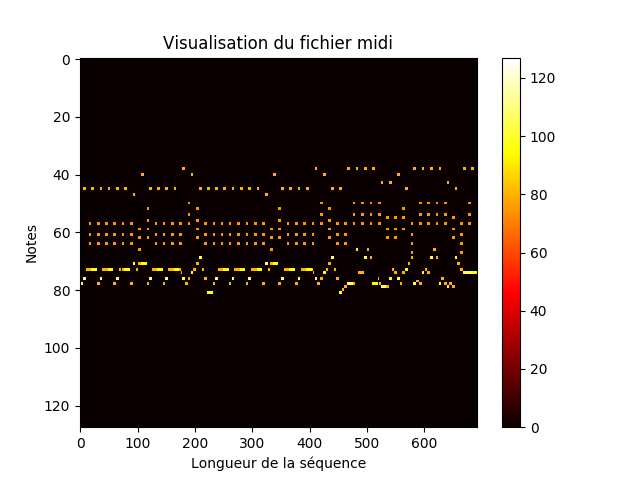
\includegraphics[width=0.5\textwidth]{images/jig1.png}\label{jig}}
  \hfill
  \subfloat[Mozart]{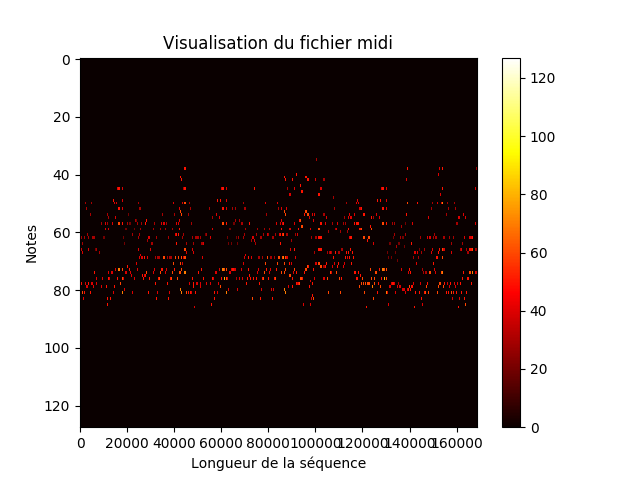
\includegraphics[width=0.5\textwidth]{images/mozart.png}\label{mozart}}
  \caption{Visualisation de fichiers midi}
\end{figure}
\end{frame}

\begin{frame}{Résultats}

\begin{figure}
\begin{center}
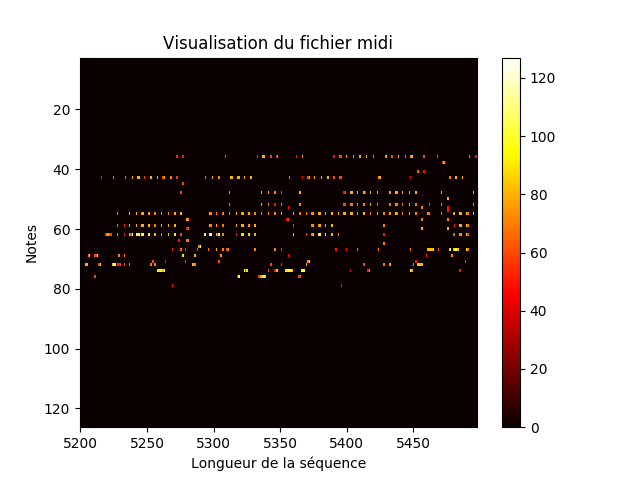
\includegraphics[width=0.5\linewidth]{images/jig_generated_38800.png}
\caption{Jig générée}
\end{center}
\end{figure}
\end{frame}

\subsection{Génération de partitions}

\begin{frame}{Génération de notes}

\end{frame}

\begin{frame}{Génération série}

\end{frame}

\begin{frame}{Génération de mesures en parallèle}

\end{frame}

\section{Conclusion}
\end{document}